\documentclass[runningheads,a4paper]{llncs}

\usepackage{amssymb}
\setcounter{tocdepth}{3}
\usepackage{graphicx}
\usepackage{subfig}

\usepackage{url}
\urldef{\mailsc}\path|{mprietopereira, m.furundarena, Nikita.Seleznev}@student.ulg.ac.be|    

\begin{document}

\title{Group 11 ErasmusKit Project Report}
\titlerunning{ErasmusKit Project Report}

\author{Mario Prieto\and Maite Furundarena\and Nikita Seleznev}
\authorrunning{Group 11}

\institute{Department of Electrical Engineering and Computer Science\\
	University of Liege\\
	Quartier Polytech 1, Sart-Tilman, Building B28, B-4000 Liege, Belgium\\
\mailsc}

\maketitle


\section{Idea}
Living overseas is always a big challenge, especially if a traveler has nobody to
meet and explain the survival basics in a new place. Being Erasmus+ \cite{erasmus_url}
students, all of group participants faced plenty problems, such as:
\begin{itemize}
	\item inability to find affordable restaurants and shops;
	\item bus ticket price (2.40 euro!), lack of information about discounts;
	\item loneliness in the early days.
\end{itemize}
Needless to say, that University of  Liege's website provides \cite{ulg_brochure} first steps
instructions for newcomers, however not every Erasmus host university provides it.
Moreover, era of mobile devices is already here, Android~$^{\tiny{\textregistered}}$	application allows
to access an important information in much appropriate way. And what's vitally
important while traveling in another country, the information could be retrieved
without internet connection.

All the things above considered pushed us to create an application for Erasmus
students all around the world.


\section{Brief overview}
The very first thing user faces in the application is welcome screen (see
Figure~\ref{fig:welcome}), offering to proceed a registration using Google account
(Figure~\ref{fig:google}) or in more traditional way using email and password 
(Figure~\ref{fig:reg}). In the case user would be notified that confirmation code
was sent to specified address; once confirmation link opened in browser, user
becomes able to log in with the credentials.

After successful authentication screen with list of cities appears as shown in
Figure~\ref{fig:cities}. Even on old devices with Holo design themes application
itself looks the same (Figure~\ref{fig:cities_tablet}) thanks to support libraries.
Figure~\ref{fig:cities_tablet} shows city search feature -- when user taps magnifier
button, keyboard appears, then letter-by-letter list of cities filters on the fly.
Finally, if user has administrative permissions, it allows him to add new city,
as shown in Figure~\ref{fig:cities_new}. Floating action '+' button becomes visible as well as remove buttons for every city. After clicking add button the following pop-up dialogue appears.

Choosing city by tap, we move to the next screen (Figure~\ref{fig:city}), where
current city could be added in favorites list, and number of sections available:
\begin{itemize}
	\item Figure~\ref{fig:city_events} -- Upcoming events (TODO fb)
	\item Figure~\ref{fig:city_people} -- List of people, (TODO) joined the network,
		thus willing to communicate with others, the people who could help newcomers
	\item Figure~\ref{fig:city_places} -- Set of places, recommended by local 
		community (TODO)
	\item Figure~\ref{fig:city_tips} -- Number of useful survival tips
\end{itemize}

\begin{center}
	\begin{figure}
		\begin{tabular}{ccc}
			\subfloat[Welcome screen]{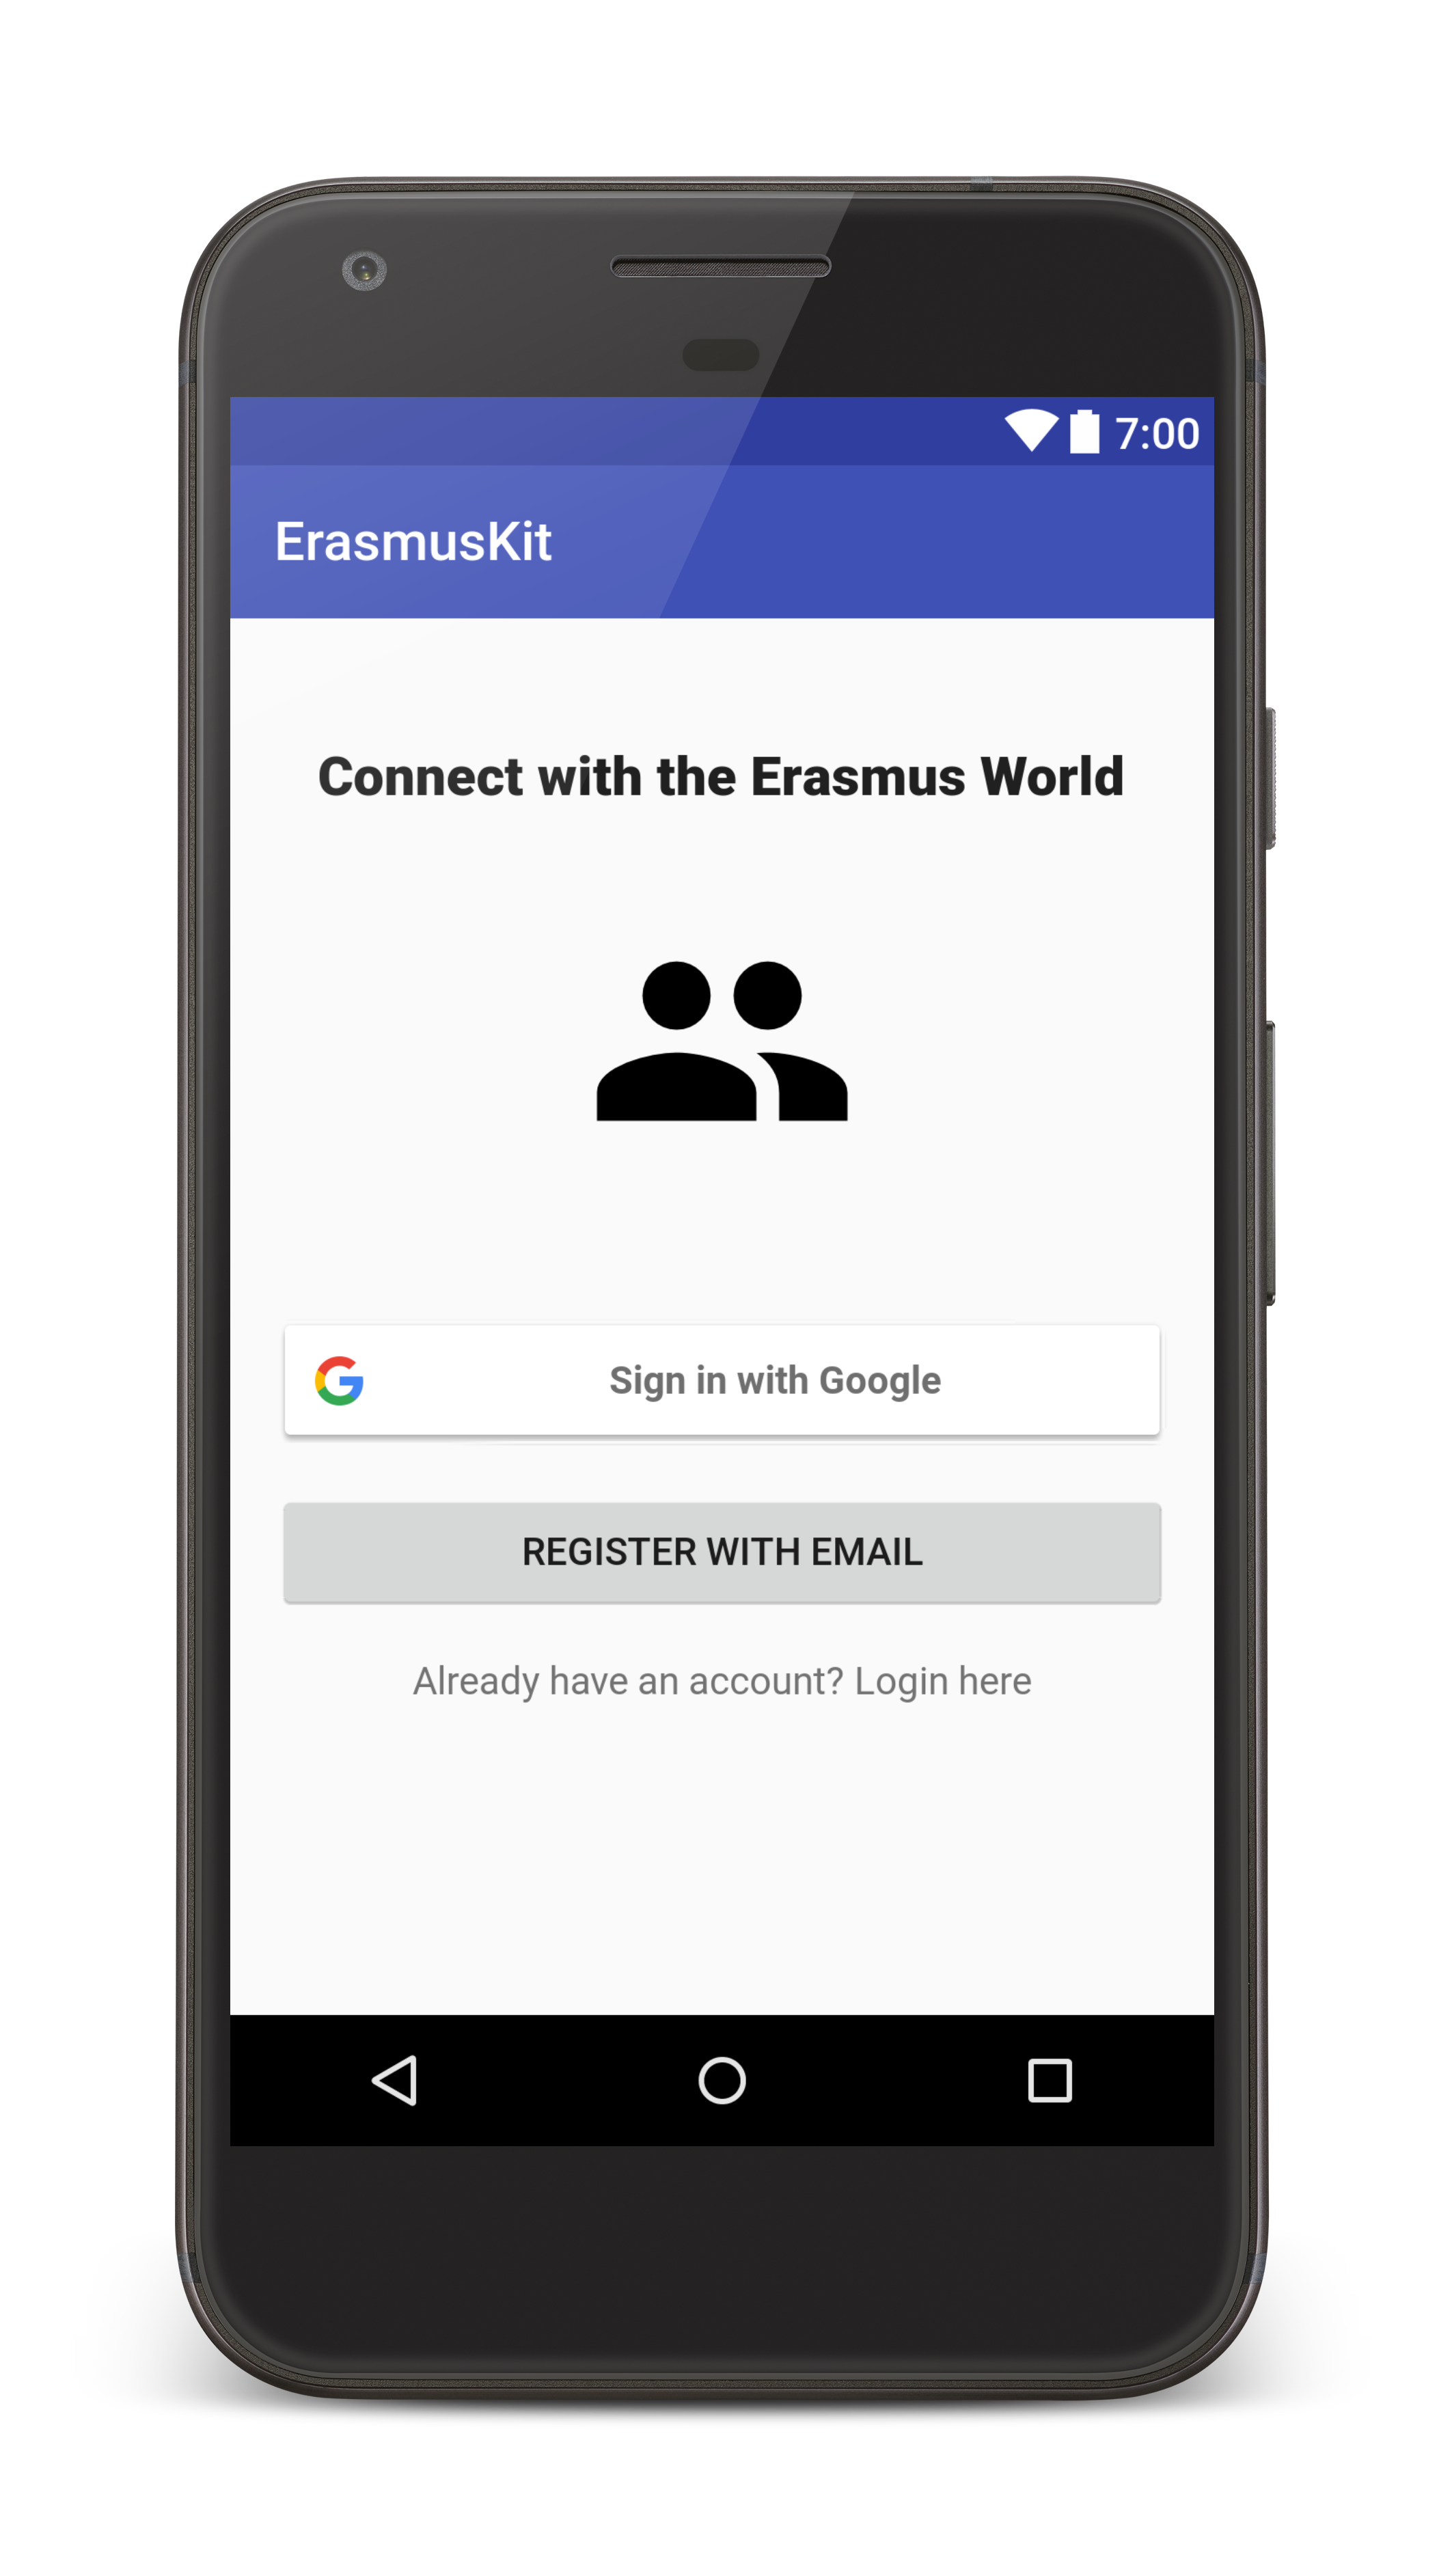
\includegraphics[width = 1.55in]{img/screen_welcome_nexus6p-portrait.png}\label{fig:welcome}} &
			\subfloat[Google login screen]{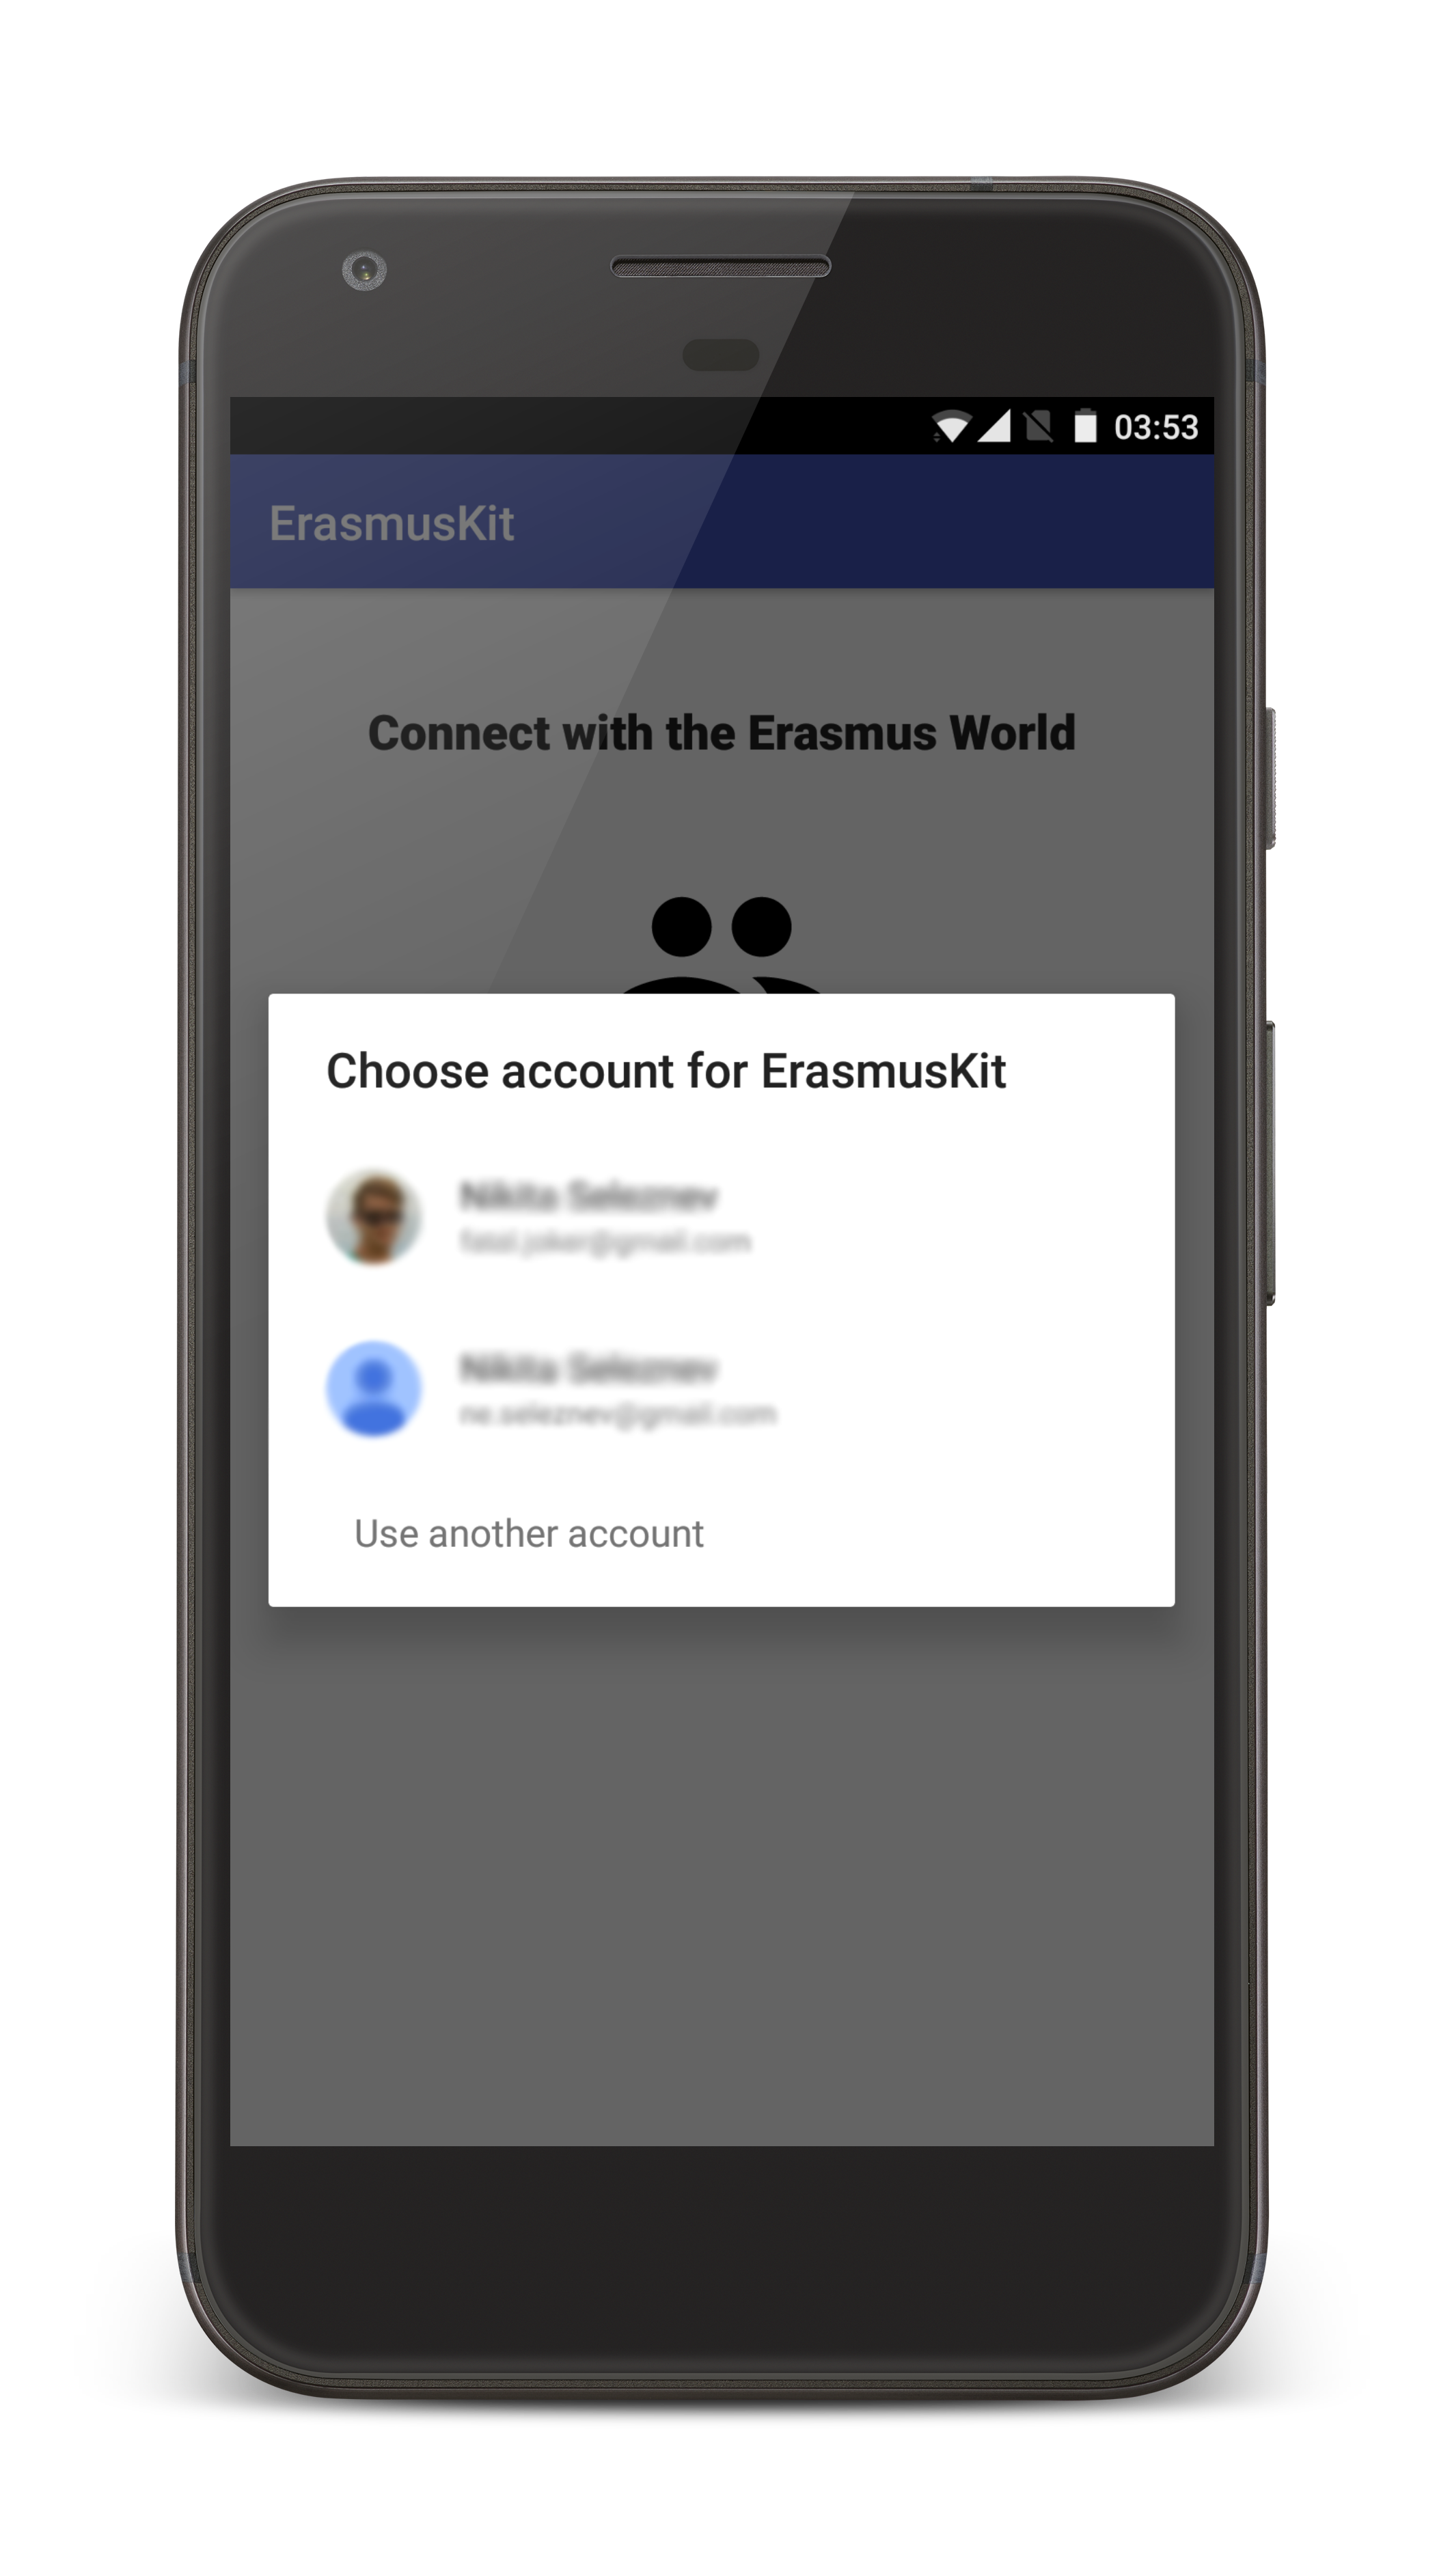
\includegraphics[width = 1.55in]{img/screen_login_nexus6p-portrait.png}\label{fig:google}} &
			\subfloat[Registration screen]{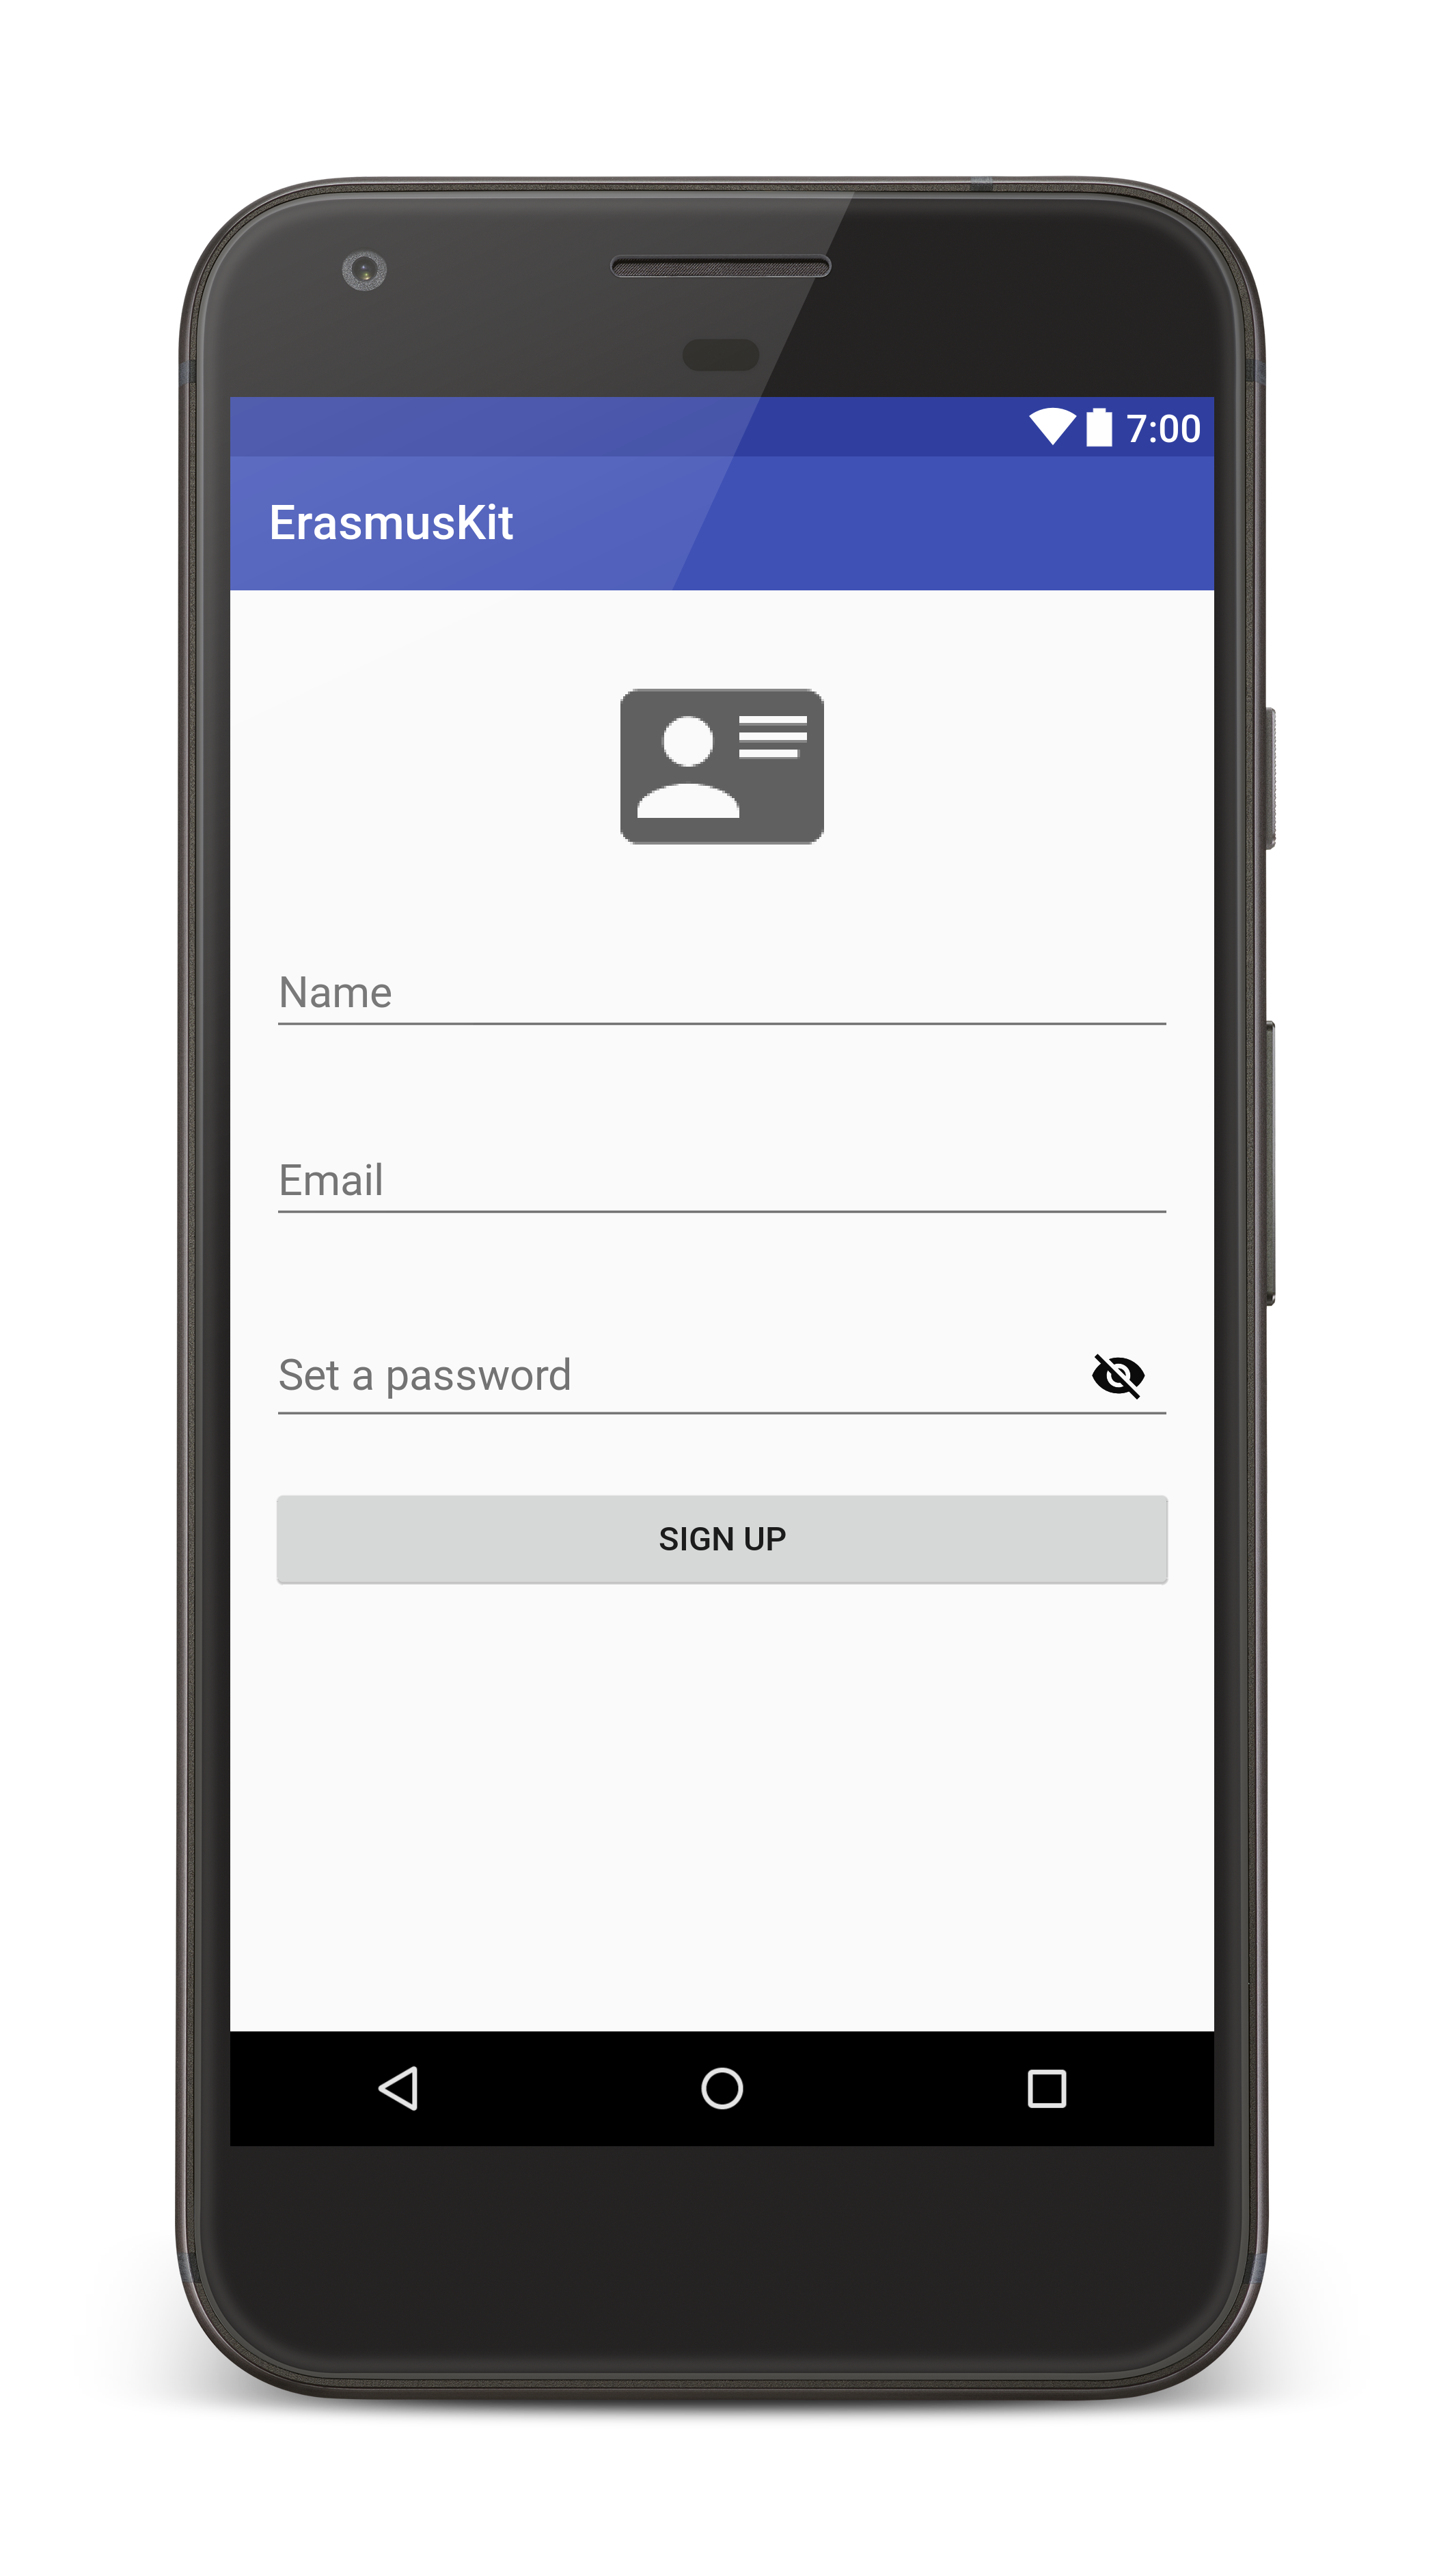
\includegraphics[width = 1.55in]{img/screen_registration_nexus6p-portrait.png}\label{fig:reg}}
		\end{tabular}
		\caption{First activities}
		\label{figure:first_activity}
	\end{figure}	
\end{center}

\begin{center}
	\begin{figure}
		\begin{tabular}{ccc}
			\subfloat[Cities acivity]{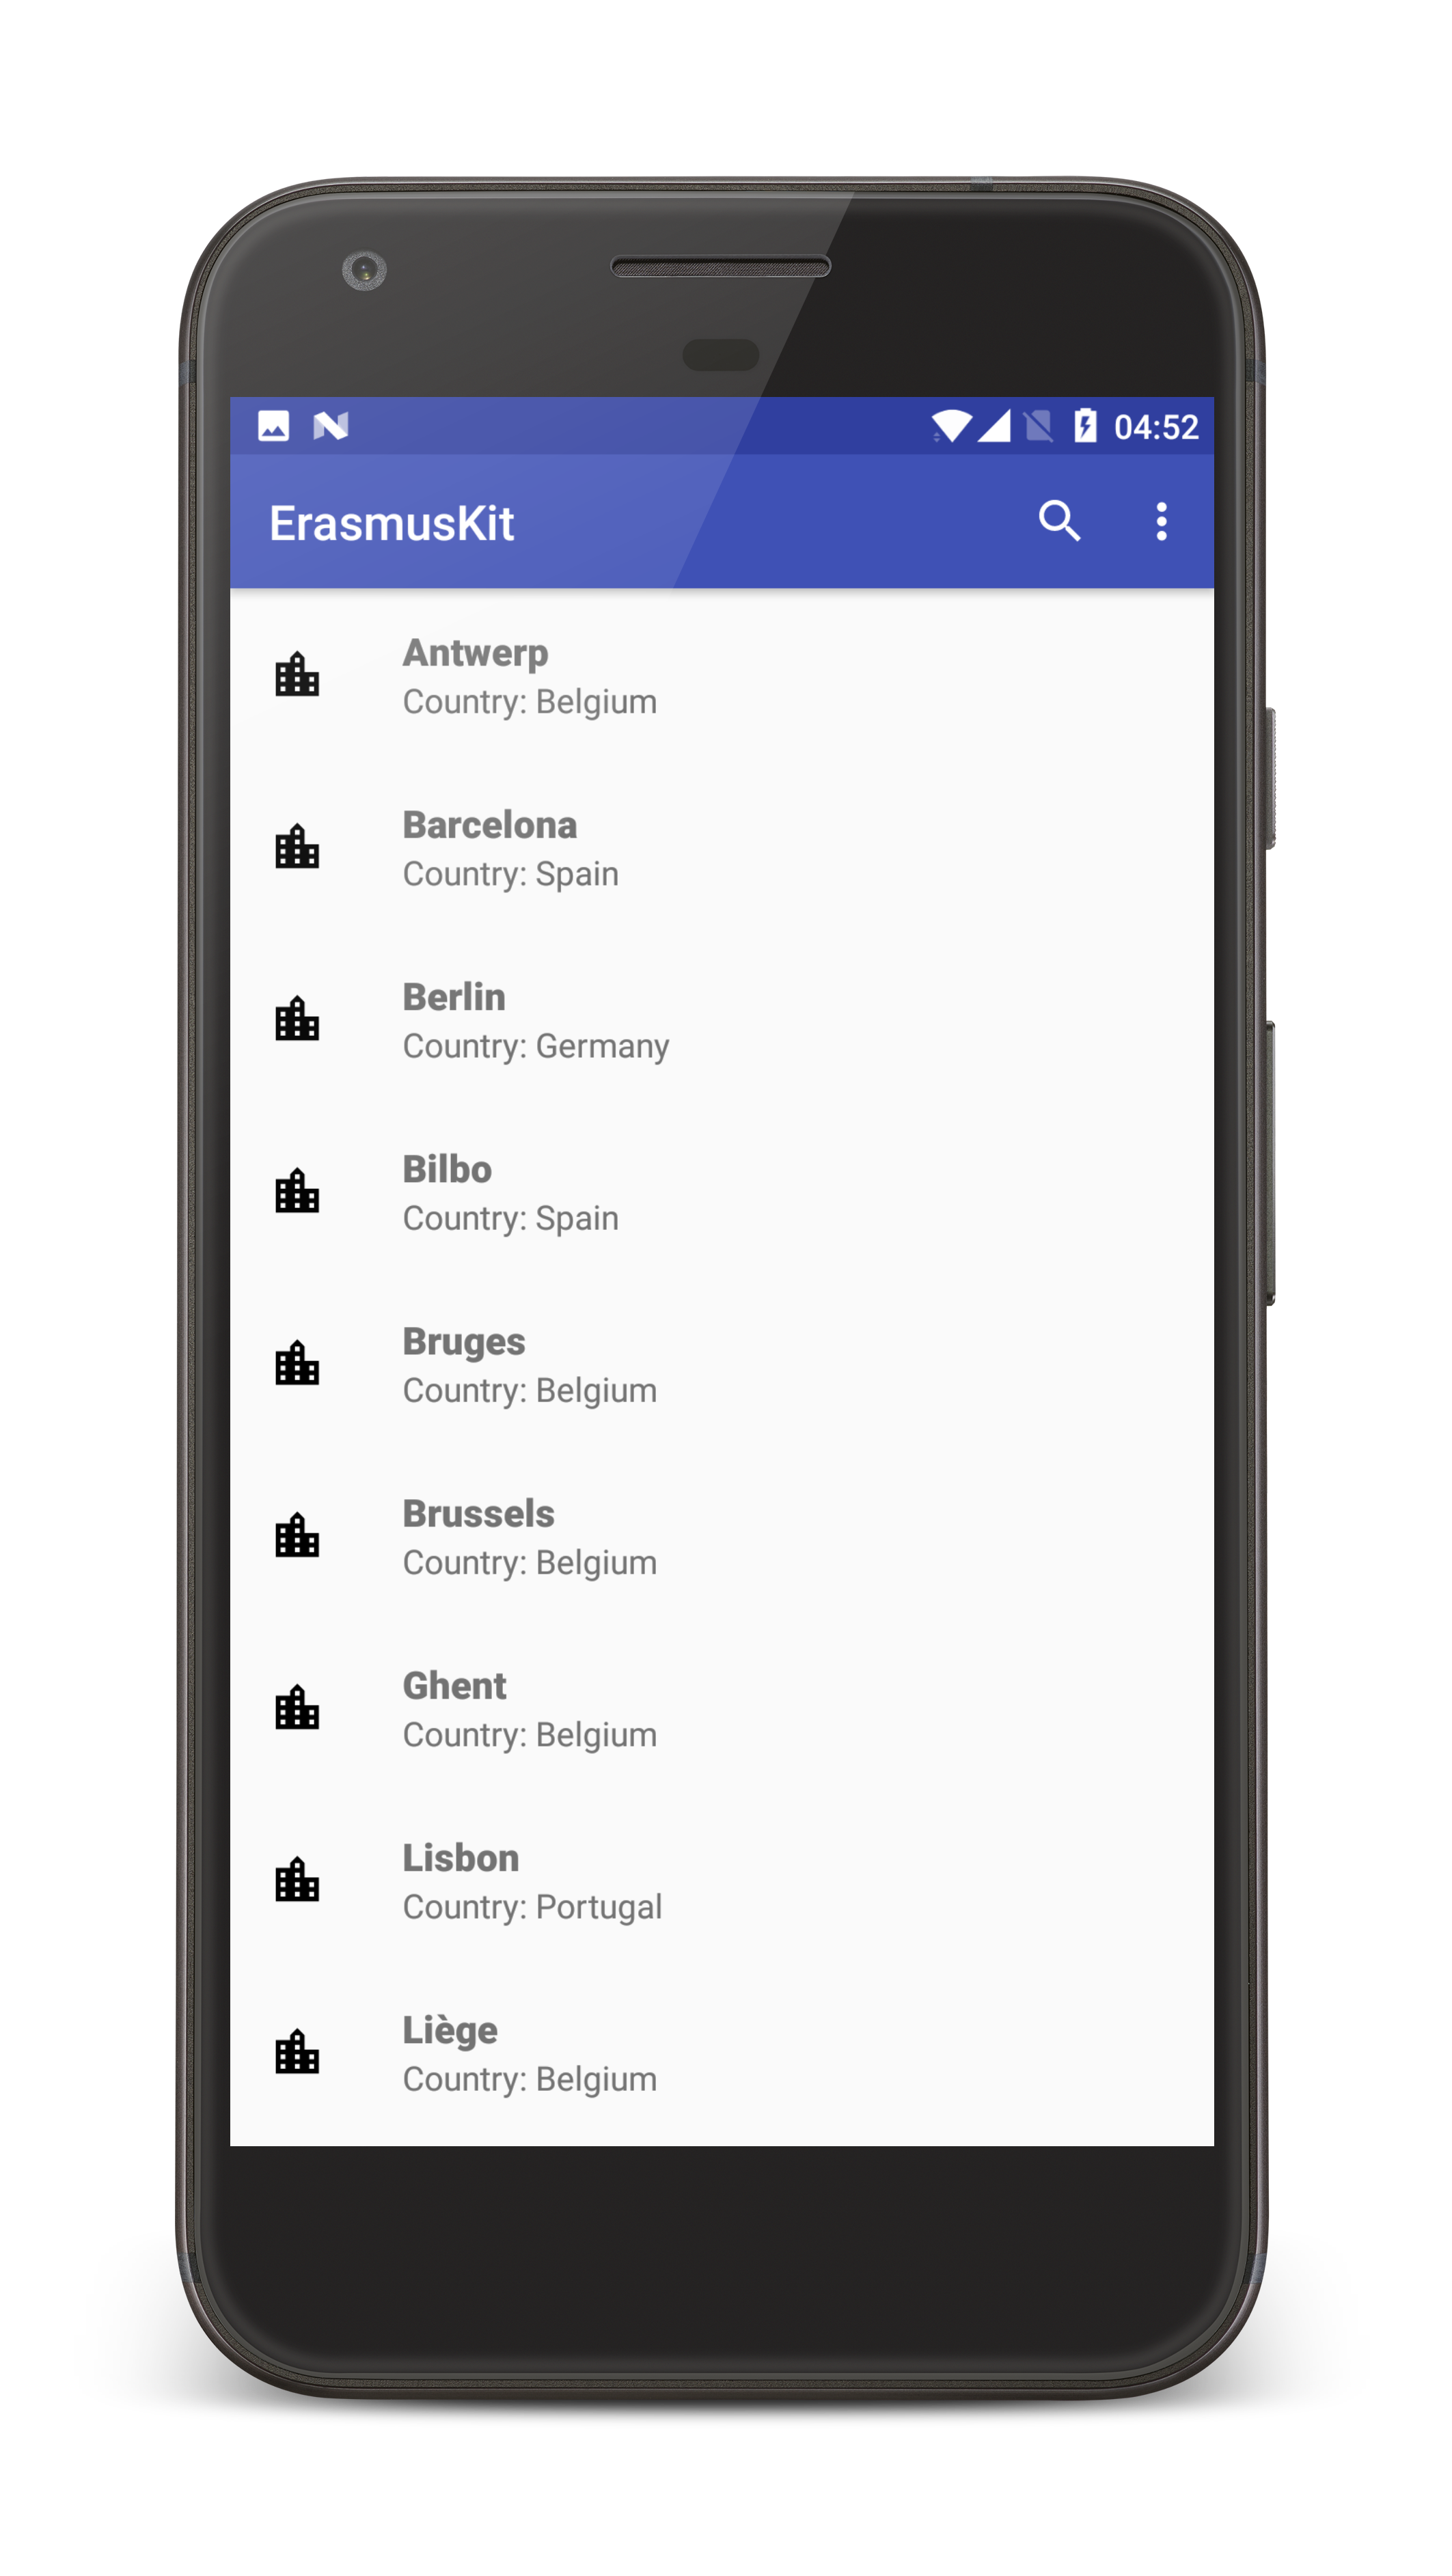
\includegraphics[width = 1.55in]{img/screen_cities_user_pixel.png}\label{fig:cities}} &
			\subfloat[Search city fragment]{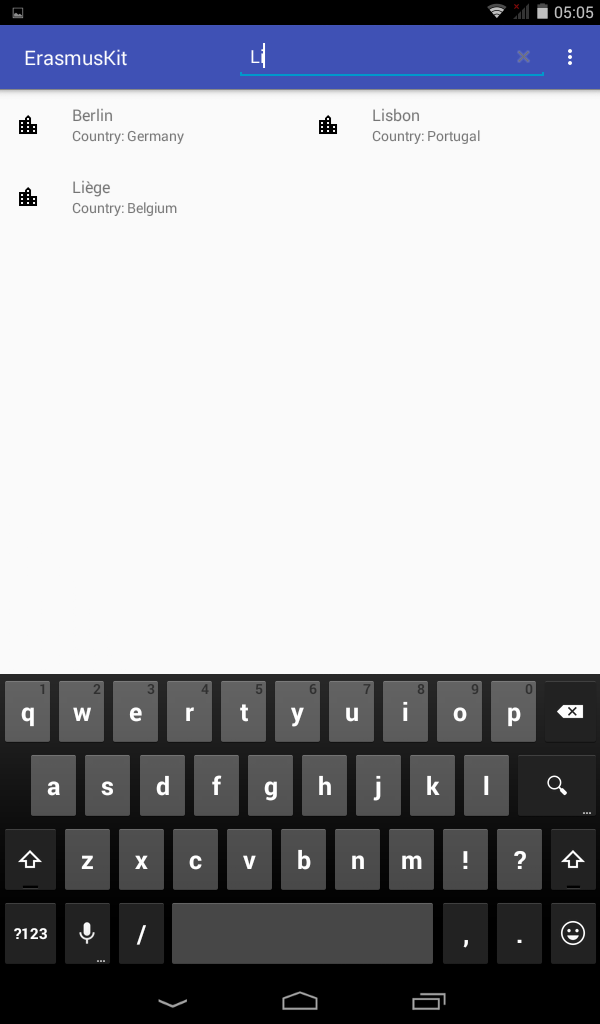
\includegraphics[width = 1.55in]{img/screen_cities.png}\label{fig:cities_tablet}} &
			\subfloat[Adding new city]{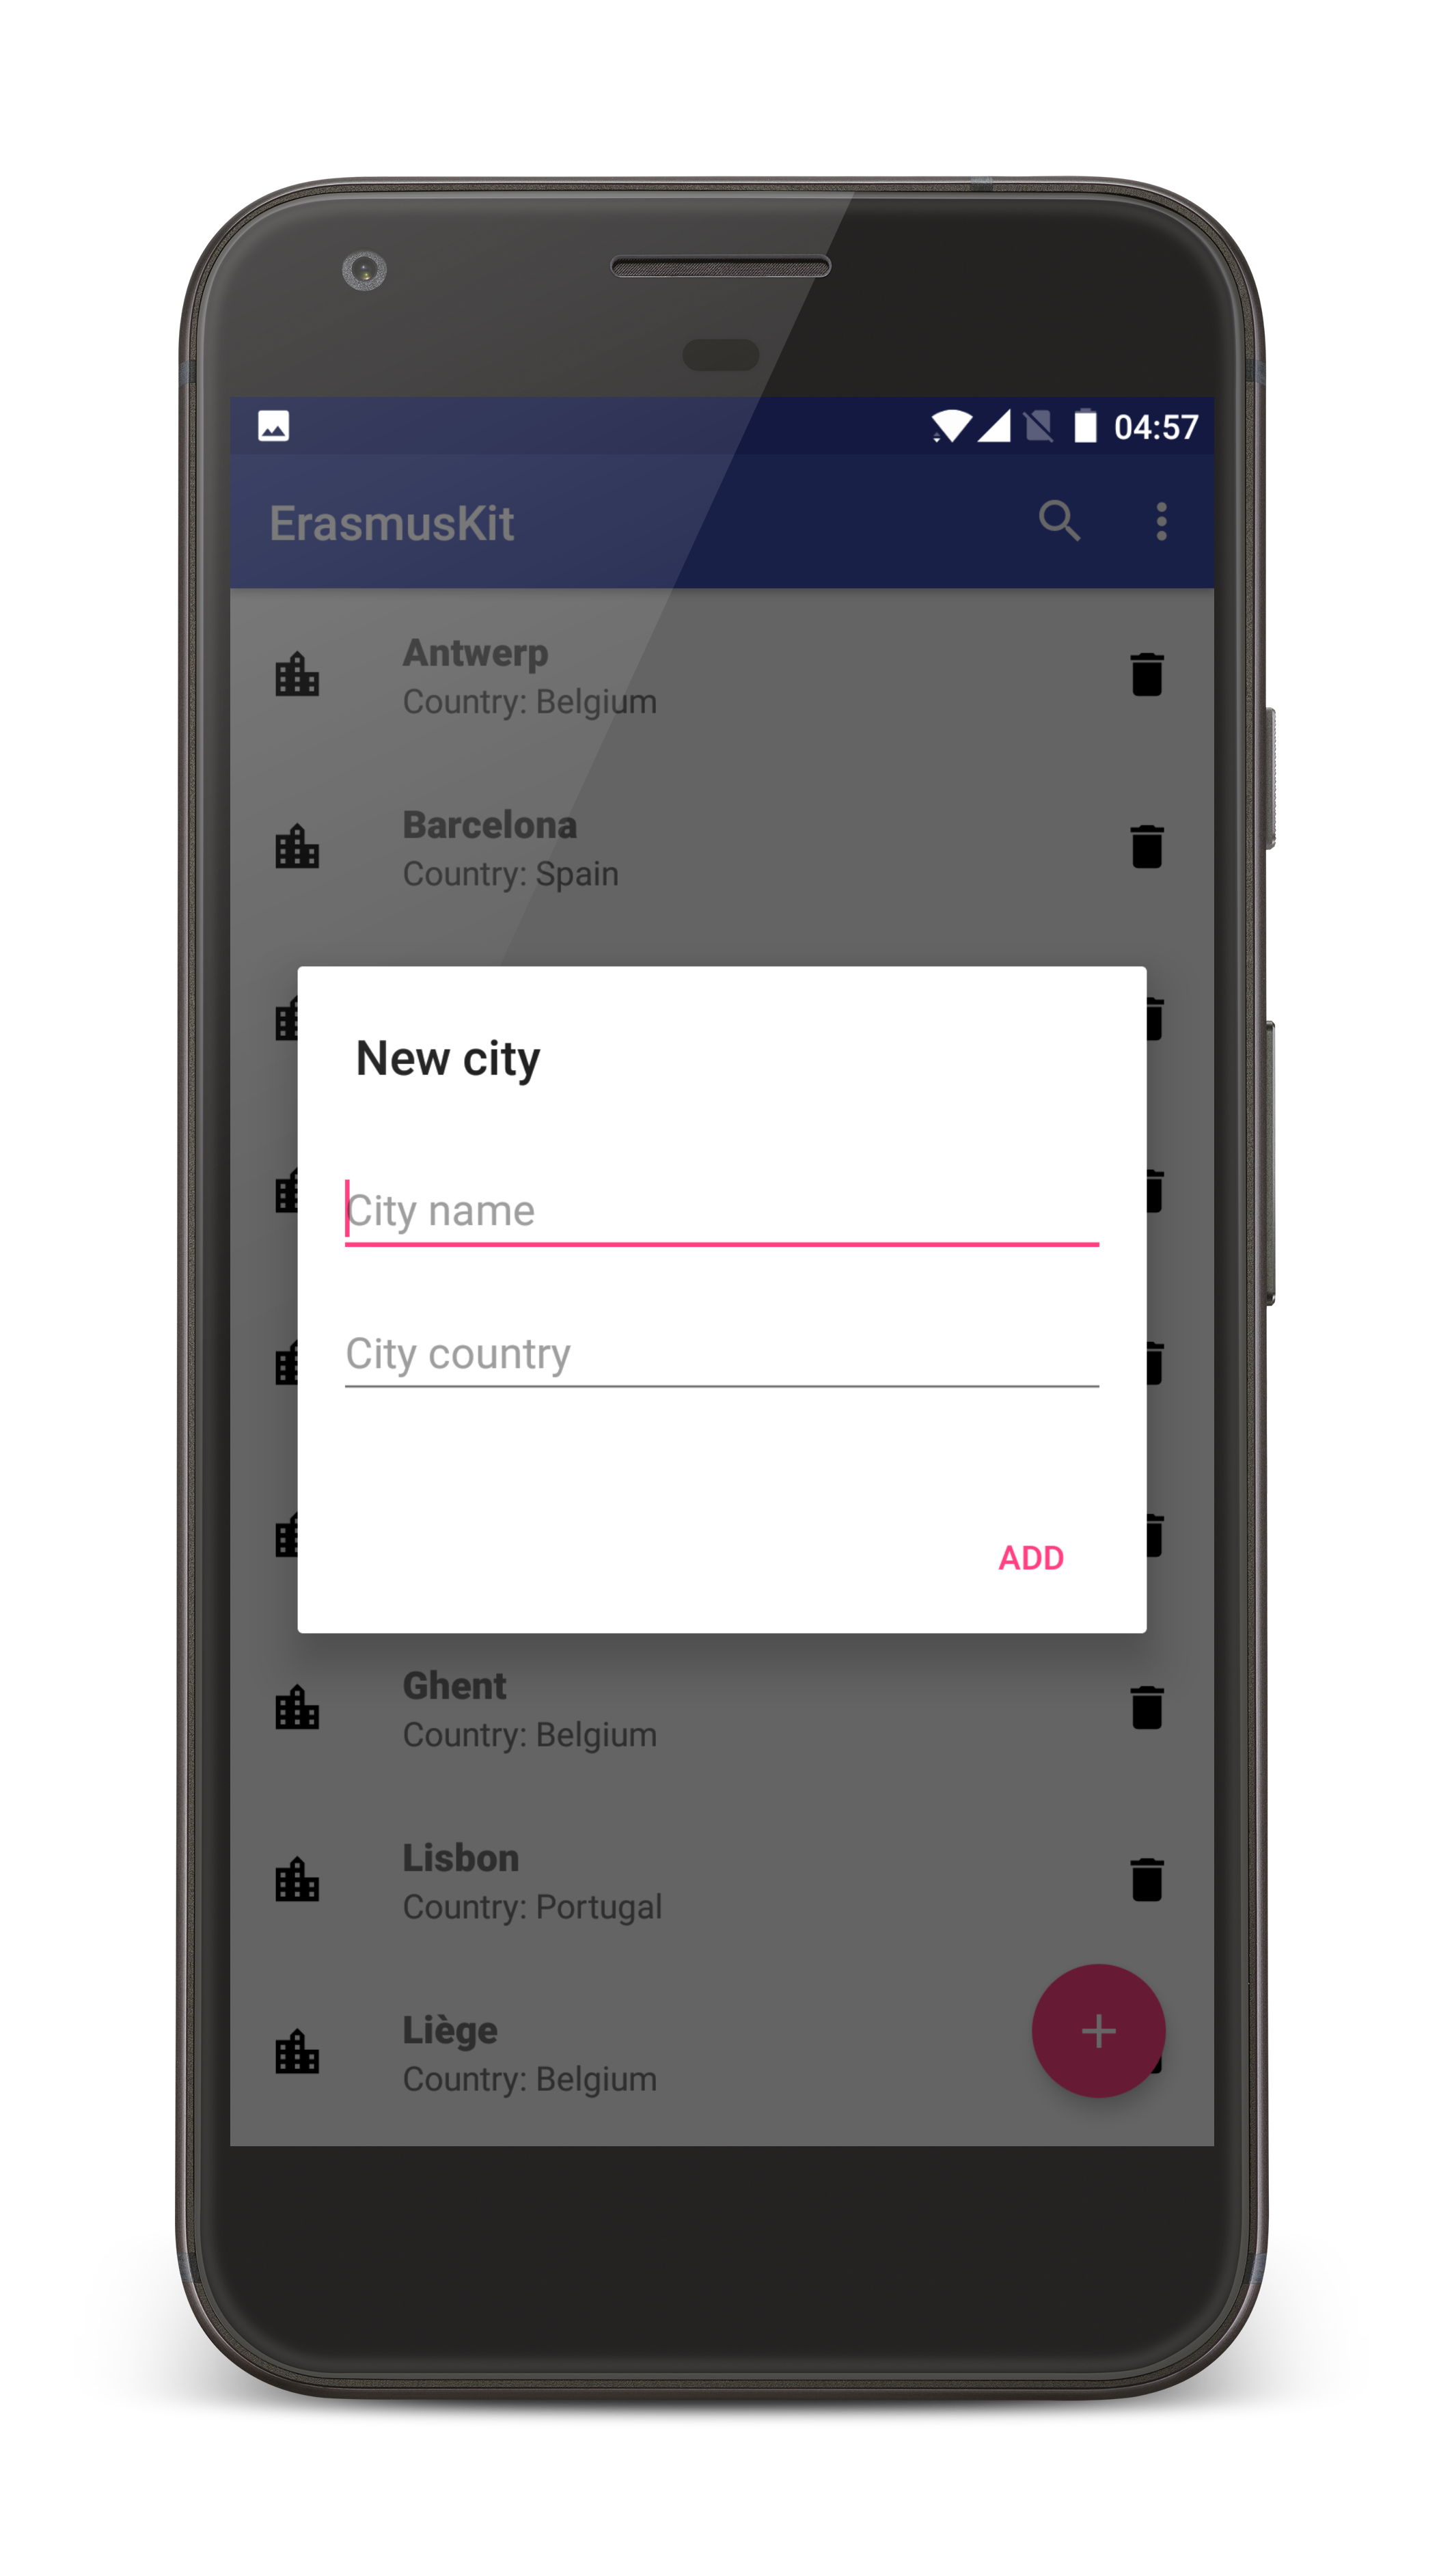
\includegraphics[width = 1.55in]{img/screen_cities_new_pixel.png}\label{fig:cities_new}}
		\end{tabular}
		\caption{Cities acivities}
		\label{figure:cities_activity}
	\end{figure}	
\end{center}

\begin{center}
	\begin{figure}
		\begin{tabular}{ccc}
			\subfloat[City screen]{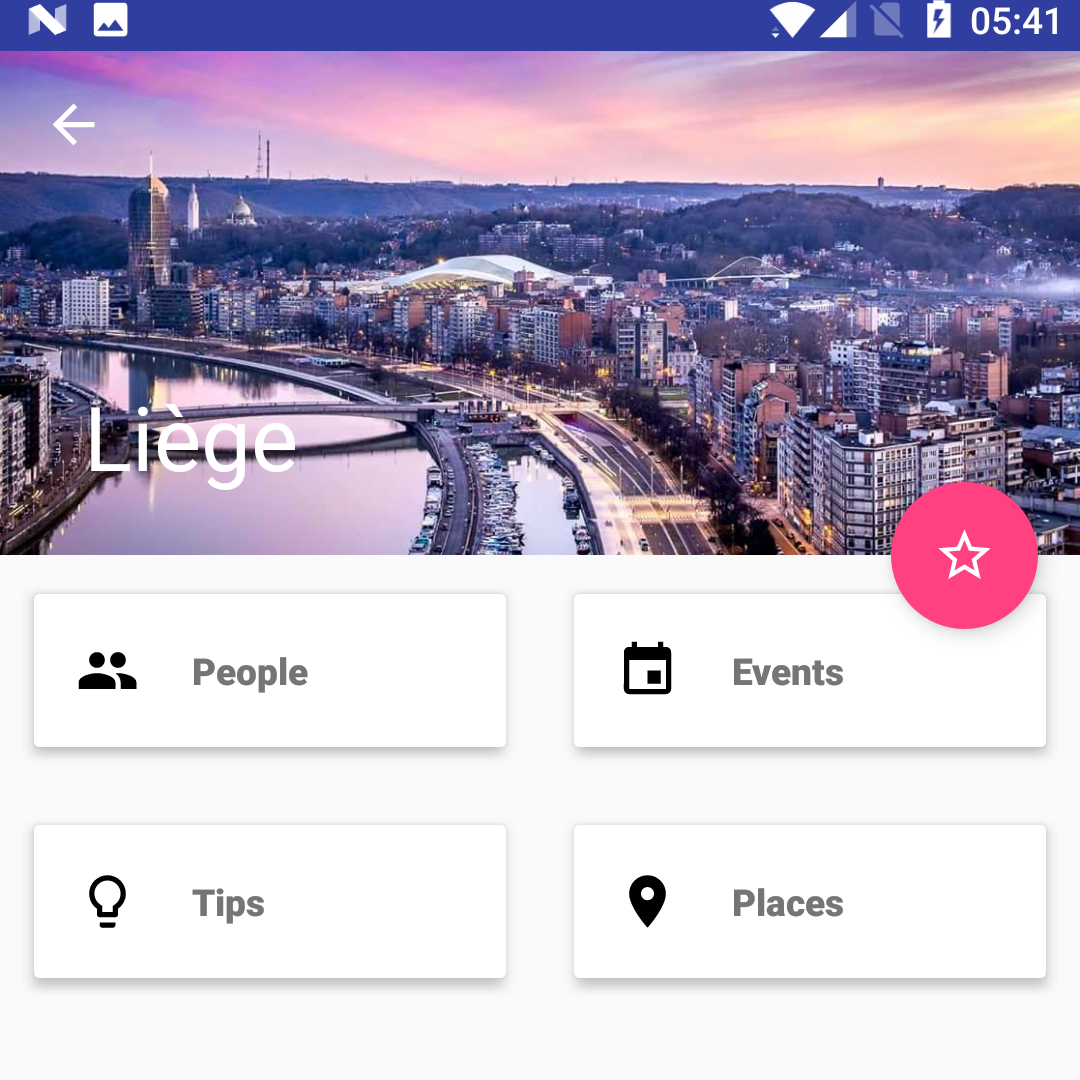
\includegraphics[width = 1.55in]{img/screen_city.png}\label{fig:city}} &
			\subfloat[City events]{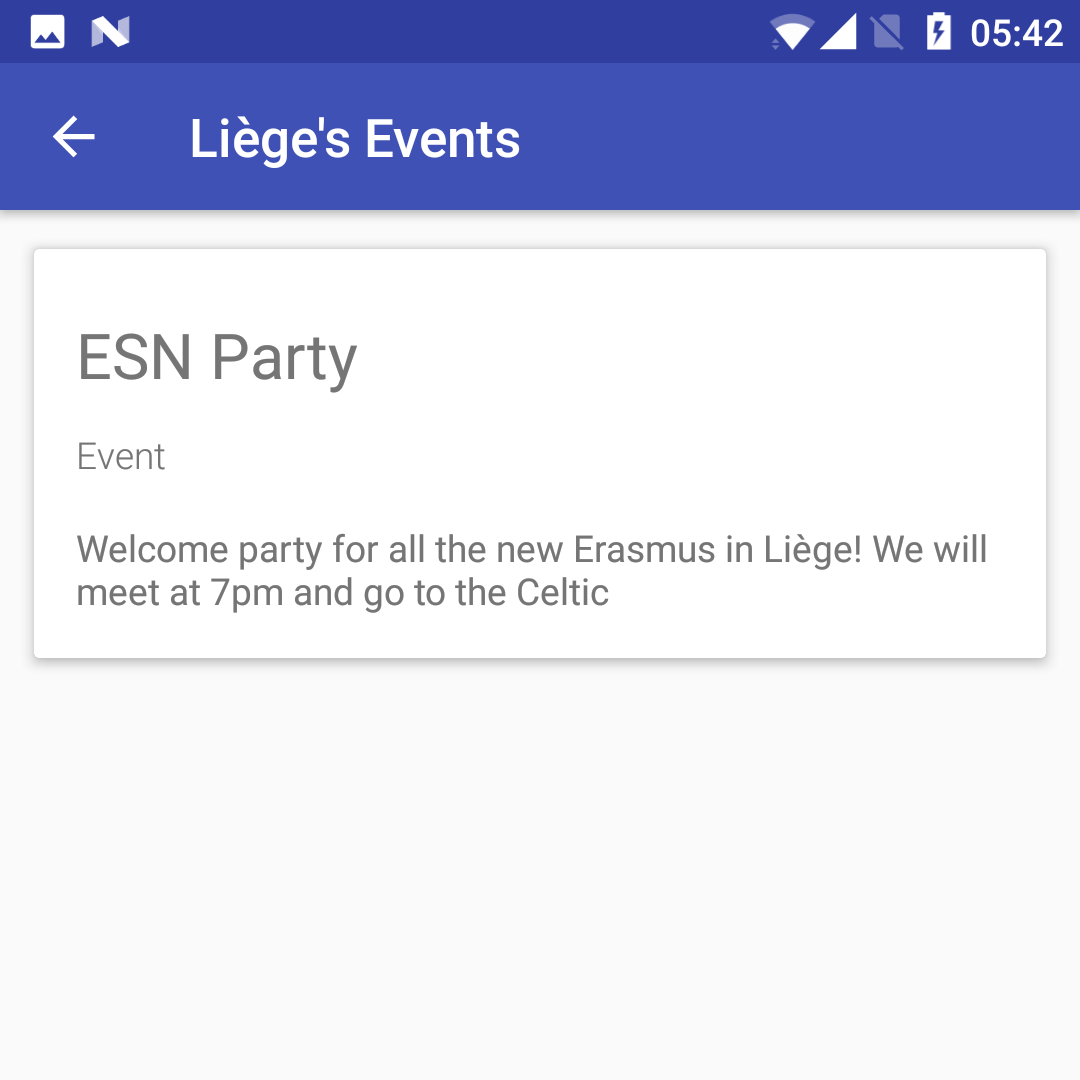
\includegraphics[width = 1.55in]{img/screen_city_events.png}\label{fig:city_events}} &
			\subfloat[People]{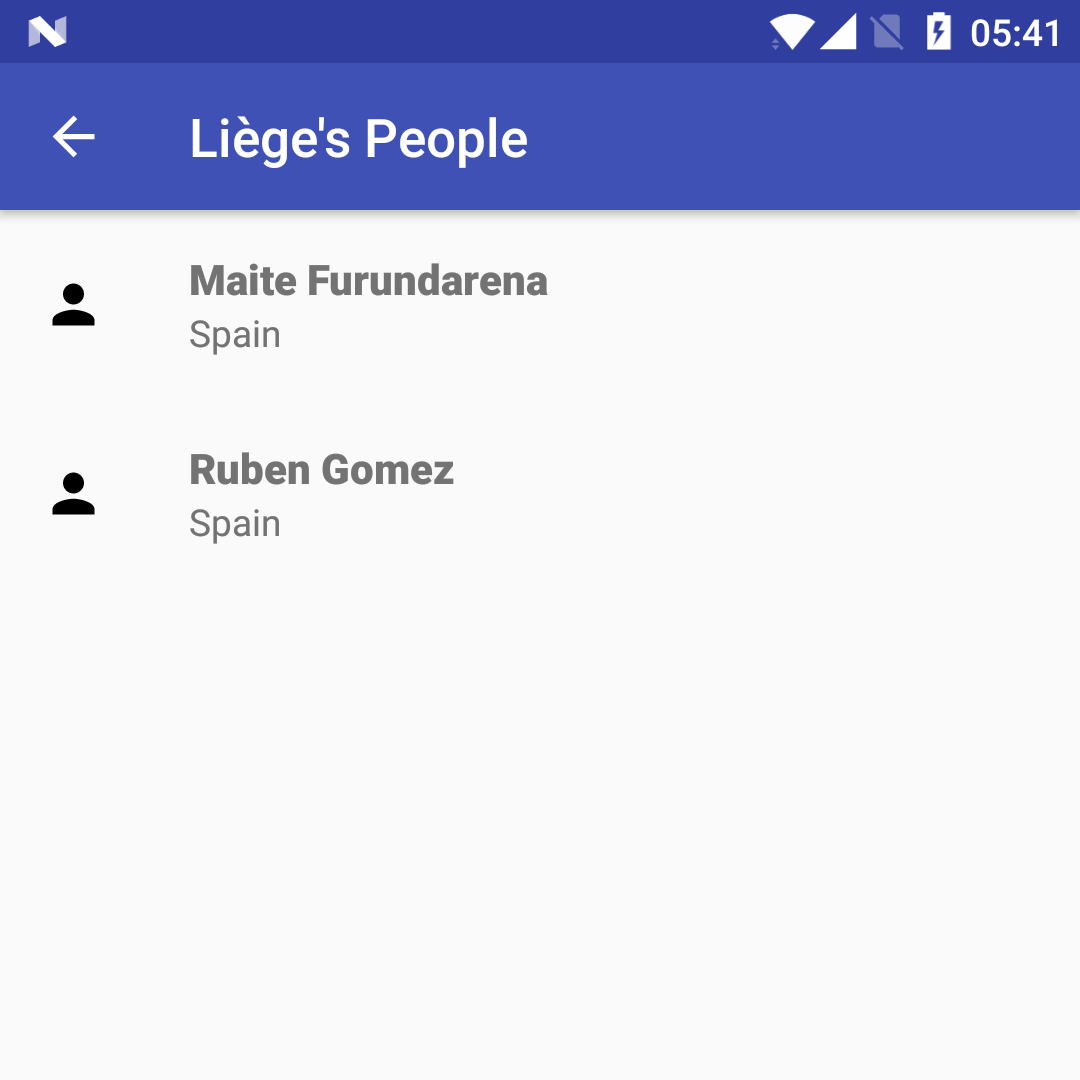
\includegraphics[width = 1.55in]{img/screen_city_people.png}\label{fig:city_people}} \\

			\subfloat[City places]{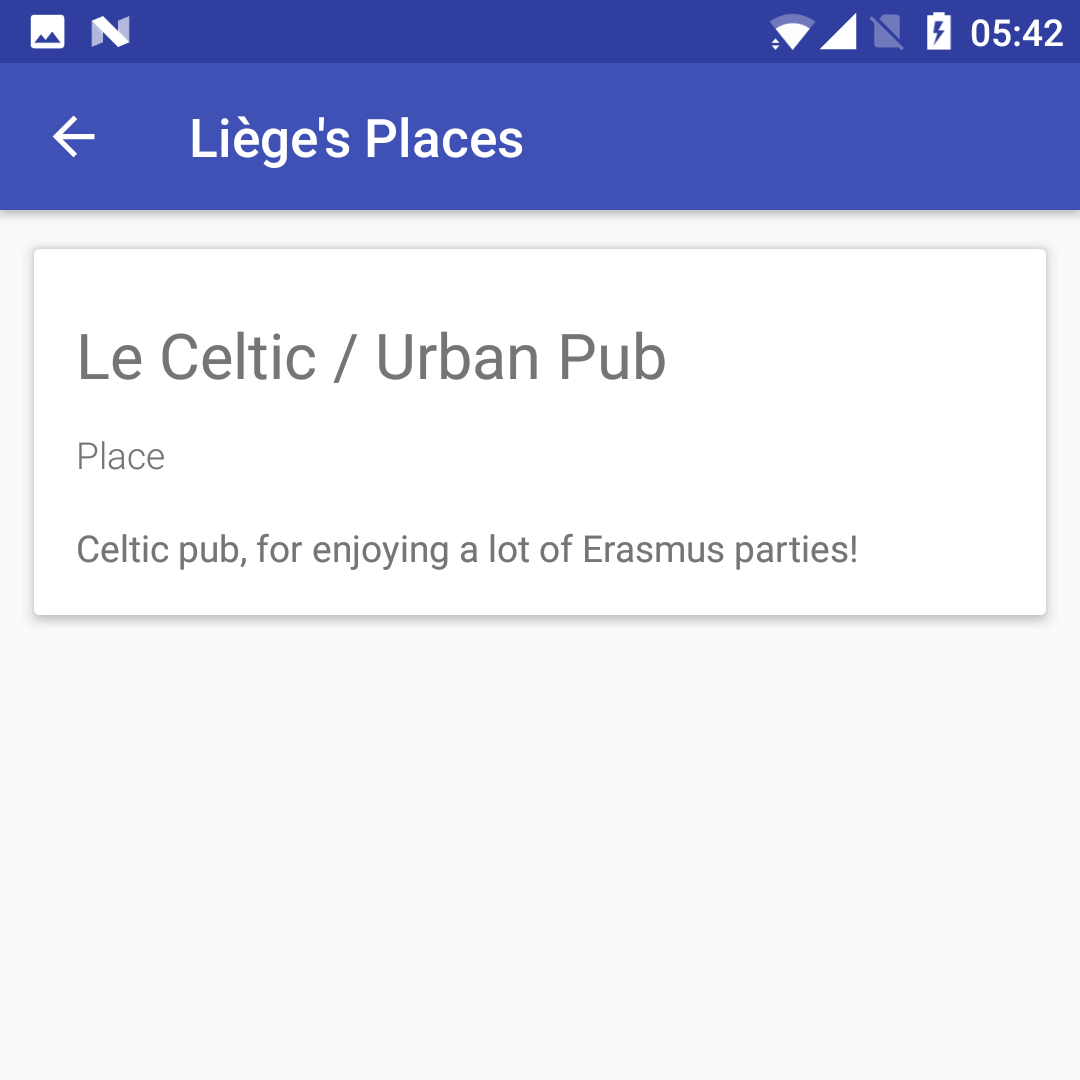
\includegraphics[width = 1.55in]{img/screen_city_places.png}\label{fig:city_places}} &
			\subfloat[City tips]{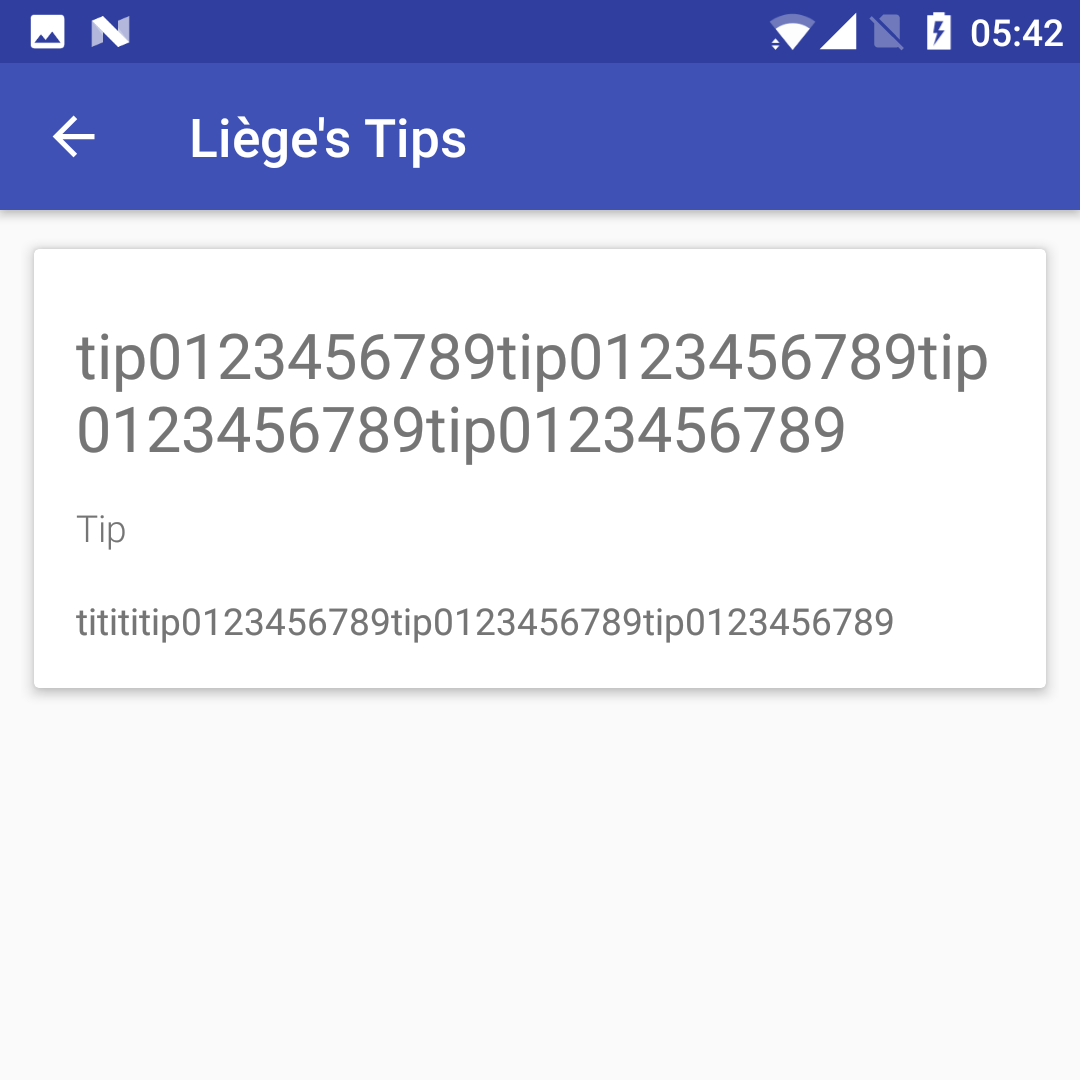
\includegraphics[width = 1.55in]{img/screen_city_tips.png}\label{fig:city_tips}} 
		\end{tabular}
		\caption{City's activities}
		\label{figure:city_activity}
	\end{figure}	
\end{center}



\section{Application components}

\subsection{Backend}
In order to provide at least accounting services application must have a server,
capable to store profile information and role. One of possible BaaS (Backend as
a Service) solutions, \texttt{Firebase} \cite{firebase} provides rich
documentation, web console, and finally Android SDK developed by Google Inc.,
so could be considered as most appropriate dummy backend for our purposes.

Following Firebase featured were enabled (included as dependencies in Gradle script):
\begin{itemize}
	\item Google services integration \texttt{com.google.gms:google-services:3.0.0};
	\item authentication \texttt{com.google.firebase:firebase-auth:10.2.1};
	\item database connection wrapper\\
		\texttt{com.google.firebase:firebase-database:10.2.1}.
\end{itemize}

In the Firebase platform itself (web console) a list of dummy features was
developed (enabled): registration (via email), authentication, and realtime
database. Figure~\ref{figure:firebase_db} shows a screenshot of database tree on 
the Firebase website. By default database allows all CRUD (create, read, update,
and delete) operations, but they were restricted by rules, for instance, only
administrator (see User roles in section TODO below) is able to do everything,
students have only read permissions, except their own profile information.

\begin{center}
	\begin{figure}
		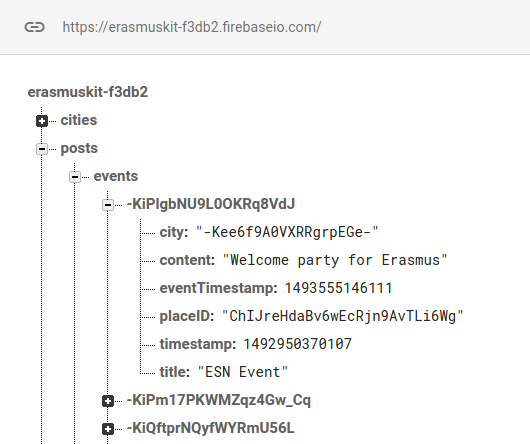
\includegraphics[width = 4.8in]{img/firebase_db.png}
		\caption{Firebase database tree with dummy elements}
		\label{figure:firebase_db}
	\end{figure}	
\end{center}

Note that Firebase SDK requires a device running Android 4.0 (Ice Cream Sandwich)
or newer, and Google Play services 10.2.1 or higher \cite{firebase_sdk}, hence
minimum API in the application became at least 14.

\subsection{User interface \& user experience}

An application is designed according to material design guidelines \cite{material}.
Material design is a comprehensive guide for visual, motion, and interaction design
across platforms and devices. Android now includes support for material design apps,
moreover there is backward compatibility achieved through support library.

The following dependencies were used in the project:
\begin{itemize}
	\item \texttt{com.android.support:appcompat-v7:25.3.1} -- this library adds
		support for the Action Bar user interface design pattern, and also includes
		support for material design user interface implementations;
	\item \texttt{com.android.support:cardview-v7:25.3.1} -- this library adds
		support for the CardView widget, which lets show information inside cards
		that have a consistent look on any app;
	\item \texttt{com.android.support:design:25.3.1} -- the Design package provides
		APIs to support adding material design components and patterns to apps.
\end{itemize}

%The new RecyclerView widget is a more pluggable version of ListView that supports different layout types and provides performance improvements.
%
%The new CardView widget lets you display important pieces of information inside cards that have a consistent look and feel.

Figure~\ref{figure:cities_activity2} shows cities activity, and, in particular,
two features: (a) how list of cities reflects orientation changement; (b) floating
action button.

In both portrait~\ref{cities_portrait} and landscape~\ref{cities_landscape}
orientations number of columns, representing city list depends on screen width.
In details, TODO Mario TODO \texttt{GridLayoutManager} 
instantiates with the number of columns, computed by formula:
$\frac{w}{d \cdot 520}$, where $w$ is display width (in pixels), given by \\
\texttt{getResources().getDisplayMetrics().widthPixels} property, $d$ is
display density, given by \texttt{getResources().getDisplayMetrics().density}
property. The number $520$ got from random table of magic numbers to fit the city list item.
The best practices of different screens handling described on android website
\cite{android_screens}.

%This rule is checked on client side, and whether violation happened, appropriate toast appears,
%informing used how to fix the error.

According to the design guidelines, a floating action button represents the primary
action in an application \cite{material_fab}, which is adding new city on 
considered screen. Button hides with animation while list scrolled down.

\begin{center}
	\begin{figure}
		\begin{tabular}{cc}
			\subfloat[Portrait orientation]{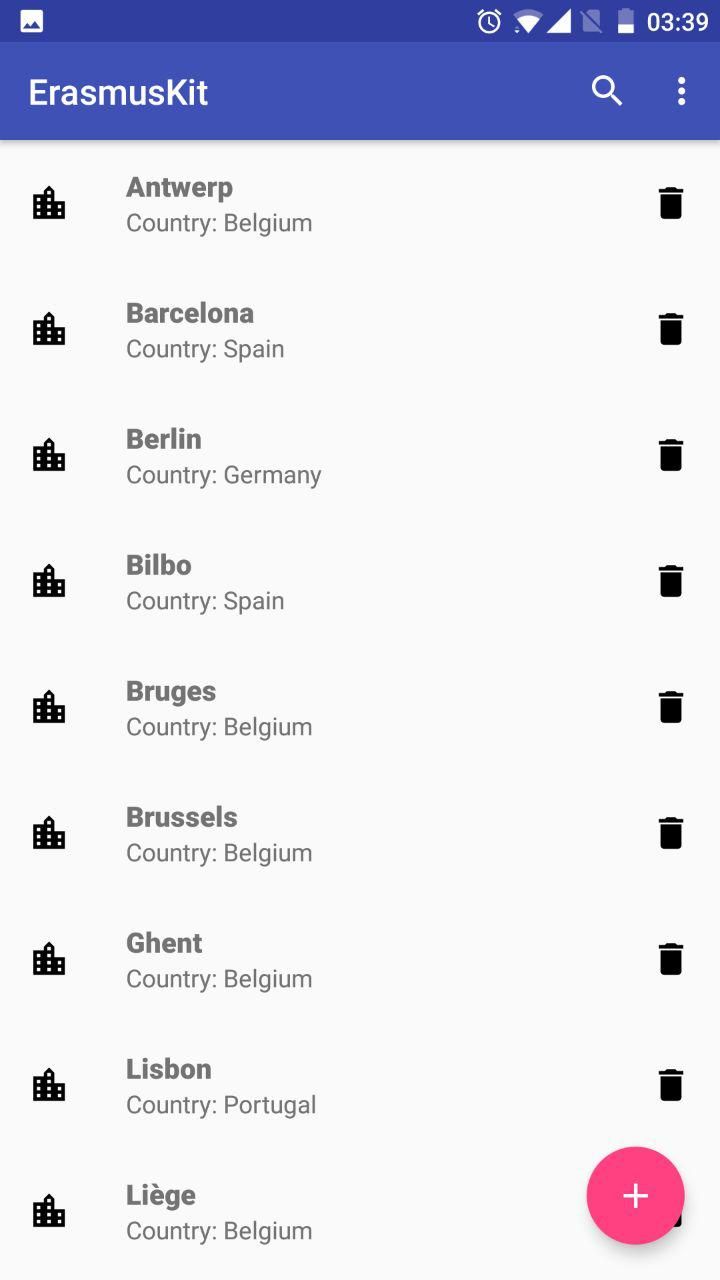
\includegraphics[height = 3in]{img/cities_activity.jpg}\label{cities_portrait}} &
			\subfloat[Landscape orientation]{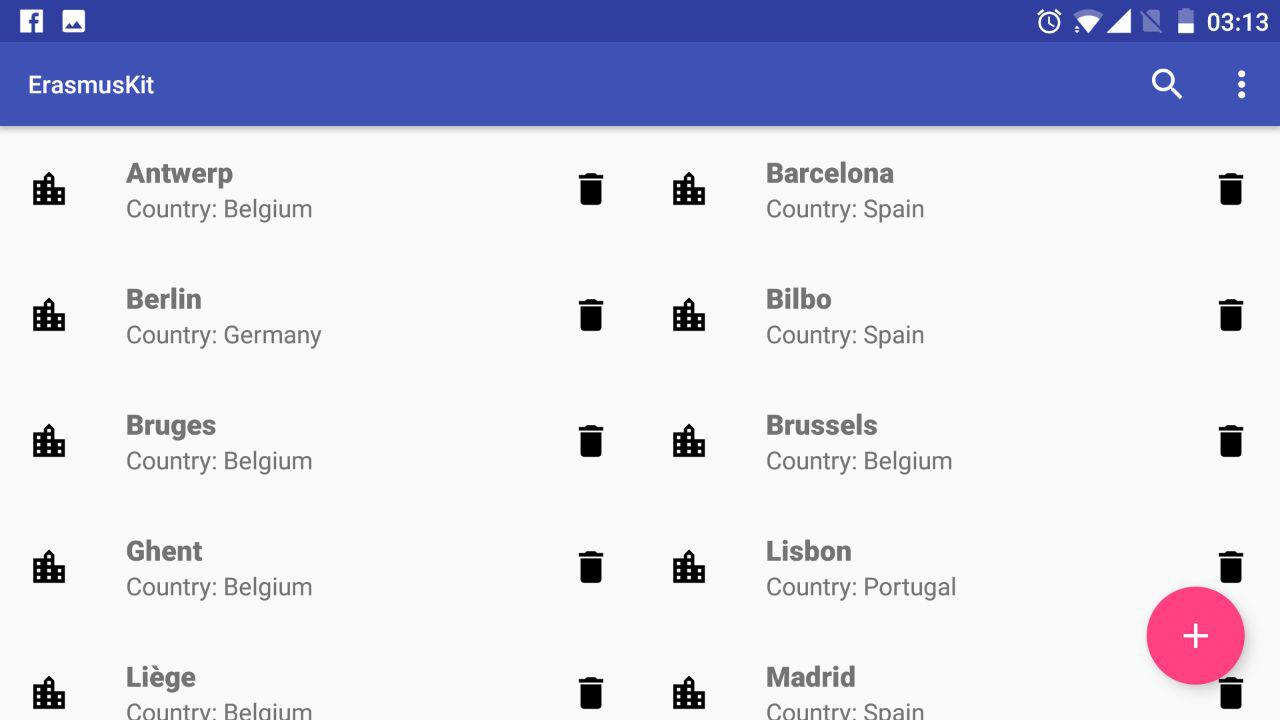
\includegraphics[width = 3in]{img/cities_activity_horizontal.jpg}\label{cities_landscape}}
		\end{tabular}
		\caption{Cities activity}
		\label{figure:cities_activity2}
	\end{figure}	
\end{center}

Used v7 Support Libraries require Android 2.3 (API level 9) and higher.

\subsection{ll}




%\begin{table}[]
%	\begin{center}
%		\begin{tabular}{| c | c | c | c | c | c | c |}
%			\hline
%			Method
%			&
%			\multicolumn{2}{c|}{1987}
%			&
%			\multicolumn{2}{c|}{1988}
%			&
%			\multicolumn{2}{c|}{1989}
%			\\ \cline{2-7}
%			
%			& ~$R^2$ value~ & Time elapsed
%			& ~$R^2$ value~ & Time elapsed
%			& ~$R^2$ value~ & Time elapsed
%			\\
%			\hline
%			
%			SLSQP 			& 0.832389 & 225  & 0.809949 & 145  & 0.906502 & 155
%			\\ \hline
%			L-BFGS-B 		& 0.829263 & 650  & 0.880573 & 865  & 0.908231 & 3493
%			\\ \hline
%			Truncated NC	& 0.832390 & 708  & 0.905172 & 993  & 0.908231 & 3474
%			\\ \hline
%			Nelder-Mead 	& 0.909165 & 2426 & 0.905333 & 4176 & 0.908246 & 5028
%			\\ \hline
%			Genetic 		& 0.832380 & 8027 & 0.902974 & 8051 & 0.908184 & 8039
%			\\
%			\hline
%		\end{tabular}
%		\caption{Time comparison for different methods for epidemic outbreak in 1987--1989}
%		\label{table:MoscowR2}
%	\end{center}
%\end{table}
%
%e.g.,
%\begin{equation}
%  \psi (u) = \int_{o}^{T} \left[\frac{1}{2}
%  \left(\Lambda_{o}^{-1} u,u\right) + N^{\ast} (-u)\right] dt \;  .
%\end{equation}
%
%Equations should be punctuated in the same way as ordinary
%text but with a small space before the end punctuation mark.
%
%\subsection{Footnotes}
%
%The superscript numeral used to refer to a footnote appears in the text
%either directly after the word to be discussed or -- in relation to a
%phrase or a sentence -- following the punctuation sign (comma,
%semicolon, or period). Footnotes should appear at the bottom of
%the
%normal text area, with a line of about 2~cm set
%immediately above them.\footnote{The footnote numeral is set flush left
%and the text follows with the usual word spacing.}
%
%\subsection{Program Code}
%
%Program listings or program commands in the text are normally set in
%typewriter font, e.g., CMTT10 or Courier.
%
%\medskip
%
%\noindent
%{\it Example of a Computer Program}
%\begin{verbatim}
%program Inflation (Output)
%  {Assuming annual inflation rates of 7%, 8%, and 10%,...
%   years};
%   const
%     MaxYears = 10;
%   var
%     Year: 0..MaxYears;
%     Factor1, Factor2, Factor3: Real;
%   begin
%     Year := 0;
%     Factor1 := 1.0; Factor2 := 1.0; Factor3 := 1.0;
%     WriteLn('Year  7% 8% 10%'); WriteLn;
%     repeat
%       Year := Year + 1;
%       Factor1 := Factor1 * 1.07;
%       Factor2 := Factor2 * 1.08;
%       Factor3 := Factor3 * 1.10;
%       WriteLn(Year:5,Factor1:7:3,Factor2:7:3,Factor3:7:3)
%     until Year = MaxYears
%end.
%\end{verbatim}
%%
%\noindent
%{\small (Example from Jensen K., Wirth N. (1991) Pascal user manual and
%report. Springer, New York)}
%
%\subsection{Citations}
%
%For citations in the text please use
%square brackets and consecutive numbers: \cite{jour}, \cite{lncschap},
%\cite{proceeding1} -- provided automatically
%by \LaTeX 's \verb|\cite| \dots\verb|\bibitem| mechanism.
%
%\section{The References Section}\label{references}
%
%In order to permit cross referencing within LNCS-Online, and eventually
%between different publishers and their online databases, LNCS will,
%from now on, be standardizing the format of the references. This new
%feature will increase the visibility of publications and facilitate
%academic research considerably. Please base your references on the
%examples below. References that don't adhere to this style will be
%reformatted by Springer. You should therefore check your references
%thoroughly when you receive the final pdf of your paper.
%The reference section must be complete. You may not omit references.
%Instructions as to where to find a fuller version of the references are
%not permissible.
%
%We only accept references written using the latin alphabet. If the title
%of the book you are referring to is in Russian or Chinese, then please write
%(in Russian) or (in Chinese) at the end of the transcript or translation
%of the title.
%
%The following section shows a sample reference list with entries for
%journal articles \cite{jour}, an LNCS chapter \cite{lncschap}, a book
%\cite{book}, proceedings without editors \cite{proceeding1} and
%\cite{proceeding2}, as well as a URL \cite{url}.
%Please note that proceedings published in LNCS are not cited with their
%full titles, but with their acronyms!

\section{Dummy}

\begin{thebibliography}{4}
	%
	%\bibitem{jour} Smith, T.F., Waterman, M.S.: Identification of Common Molecular
	%Subsequences. J. Mol. Biol. 147, 195--197 (1981)
	%
	%\bibitem{lncschap} May, P., Ehrlich, H.C., Steinke, T.: ZIB Structure Prediction Pipeline:
	%Composing a Complex Biological Workflow through Web Services. In: Nagel,
	%W.E., Walter, W.V., Lehner, W. (eds.) Euro-Par 2006. LNCS, vol. 4128,
	%pp. 1148--1158. Springer, Heidelberg (2006)
	%
	%\bibitem{book} Foster, I., Kesselman, C.: The Grid: Blueprint for a New Computing
	%Infrastructure. Morgan Kaufmann, San Francisco (1999)
	%
	%\bibitem{proceeding1} Czajkowski, K., Fitzgerald, S., Foster, I., Kesselman, C.: Grid
	%Information Services for Distributed Resource Sharing. In: 10th IEEE
	%International Symposium on High Performance Distributed Computing, pp.
	%181--184. IEEE Press, New York (2001)
	%
	%\bibitem{proceeding2} Foster, I., Kesselman, C., Nick, J., Tuecke, S.: The Physiology of the
	%Grid: an Open Grid Services Architecture for Distributed Systems
	%Integration. Technical report, Global Grid Forum (2002)
	%
	\bibitem{erasmus_url} Erasmus+ Studying Abroad, \url{https://ec.europa.eu/programmes/erasmus-plus/opportunities-for-individuals/students/studying-abroad_en}
	
	\bibitem{ulg_brochure} ULg's international brochure, \url{https://www.ulg.ac.be/upload/docs/application/pdf/2014-05/ulg_international_print_ok.pdf}
	
	\bibitem{firebase} Firebase by Google Inc., BaaS, \url{https://firebase.google.com/}
	
	\bibitem{firebase_sdk} Firebase Android SDK by Google Inc., \url{https://firebase.google.com/docs/android/setup}
	
	\bibitem{material} Material design guidelines, \url{https://material.io/guidelines/}
	
	\bibitem{material_fab} Material design guidelines, floating action button, \url{https://material.io/guidelines/components/buttons-floating-action-button.html}
	
	\bibitem{android_screens} Android screens support practices, \url{https://developer.android.com/guide/practices/screens_support.html}
\end{thebibliography}


\section*{Appendix}
Text

\end{document}
